\batchmode
\documentclass[twoside]{book}

% Packages required by doxygen
\usepackage{fixltx2e}
\usepackage{calc}
\usepackage{doxygen}
\usepackage[export]{adjustbox} % also loads graphicx
\usepackage{graphicx}
\usepackage[utf8]{inputenc}
\usepackage{makeidx}
\usepackage{multicol}
\usepackage{multirow}
\PassOptionsToPackage{warn}{textcomp}
\usepackage{textcomp}
\usepackage[nointegrals]{wasysym}
\usepackage[table]{xcolor}

% Font selection
\usepackage[T1]{fontenc}
\usepackage[scaled=.90]{helvet}
\usepackage{courier}
\usepackage{amssymb}
\usepackage{sectsty}
\renewcommand{\familydefault}{\sfdefault}
\allsectionsfont{%
  \fontseries{bc}\selectfont%
  \color{darkgray}%
}
\renewcommand{\DoxyLabelFont}{%
  \fontseries{bc}\selectfont%
  \color{darkgray}%
}
\newcommand{\+}{\discretionary{\mbox{\scriptsize$\hookleftarrow$}}{}{}}

% Page & text layout
\usepackage{geometry}
\geometry{%
  a4paper,%
  top=2.5cm,%
  bottom=2.5cm,%
  left=2.5cm,%
  right=2.5cm%
}
\tolerance=750
\hfuzz=15pt
\hbadness=750
\setlength{\emergencystretch}{15pt}
\setlength{\parindent}{0cm}
\setlength{\parskip}{3ex plus 2ex minus 2ex}
\makeatletter
\renewcommand{\paragraph}{%
  \@startsection{paragraph}{4}{0ex}{-1.0ex}{1.0ex}{%
    \normalfont\normalsize\bfseries\SS@parafont%
  }%
}
\renewcommand{\subparagraph}{%
  \@startsection{subparagraph}{5}{0ex}{-1.0ex}{1.0ex}{%
    \normalfont\normalsize\bfseries\SS@subparafont%
  }%
}
\makeatother

% Headers & footers
\usepackage{fancyhdr}
\pagestyle{fancyplain}
\fancyhead[LE]{\fancyplain{}{\bfseries\thepage}}
\fancyhead[CE]{\fancyplain{}{}}
\fancyhead[RE]{\fancyplain{}{\bfseries\leftmark}}
\fancyhead[LO]{\fancyplain{}{\bfseries\rightmark}}
\fancyhead[CO]{\fancyplain{}{}}
\fancyhead[RO]{\fancyplain{}{\bfseries\thepage}}
\fancyfoot[LE]{\fancyplain{}{}}
\fancyfoot[CE]{\fancyplain{}{}}
\fancyfoot[RE]{\fancyplain{}{\bfseries\scriptsize Generated by Doxygen }}
\fancyfoot[LO]{\fancyplain{}{\bfseries\scriptsize Generated by Doxygen }}
\fancyfoot[CO]{\fancyplain{}{}}
\fancyfoot[RO]{\fancyplain{}{}}
\renewcommand{\footrulewidth}{0.4pt}
\renewcommand{\chaptermark}[1]{%
  \markboth{#1}{}%
}
\renewcommand{\sectionmark}[1]{%
  \markright{\thesection\ #1}%
}

% Indices & bibliography
\usepackage{natbib}
\usepackage[titles]{tocloft}
\setcounter{tocdepth}{3}
\setcounter{secnumdepth}{5}
\makeindex

% Hyperlinks (required, but should be loaded last)
\usepackage{ifpdf}
\ifpdf
  \usepackage[pdftex,pagebackref=true]{hyperref}
\else
  \usepackage[ps2pdf,pagebackref=true]{hyperref}
\fi
\hypersetup{%
  colorlinks=true,%
  linkcolor=blue,%
  citecolor=blue,%
  unicode%
}

% Custom commands
\newcommand{\clearemptydoublepage}{%
  \newpage{\pagestyle{empty}\cleardoublepage}%
}

\usepackage{caption}
\captionsetup{labelsep=space,justification=centering,font={bf},singlelinecheck=off,skip=4pt,position=top}

%===== C O N T E N T S =====

\begin{document}

% Titlepage & ToC
\hypersetup{pageanchor=false,
             bookmarksnumbered=true,
             pdfencoding=unicode
            }
\pagenumbering{alph}
\pagenumbering{arabic}
\hypersetup{pageanchor=true}

%--- Begin generated contents ---
\chapter{Demo problem\+: Compressible and incompressible behaviour}
\label{index}\hypertarget{index}{}\hypertarget{index_q}{}\section{A few quick questions...}\label{index_q}
Since {\ttfamily oomph-\/lib} is developed as open-\/source software, any evidence that the code is being downloaded and used is very helpful for us as it helps to justify our continued work on this project.

We would therefore be extremely grateful if you could provide the information requested in the form below. Pressing the \char`\"{}submit\char`\"{} button will get you to the actual download page.

{\bfseries Note\+:} 
\begin{DoxyItemize}
\item All information will be treated as confidential. 
\item If you provide your email address and check the appropriate box we will add you to our mailing list to inform you of upgrades and bug fixes to the code. Rest assured that the mailing list is {\bfseries very low volume} -- we have better things to do than to bombard you with email. 
\item If you still feel reluctant to provide any of the information requested, feel free to enter some dummy input. The form will check that {\bfseries some} information has been entered but entering your name as \char`\"{}\+Joe Cool\char`\"{} is perfectly acceptable -- this is to discourage people from not providing the information simply because they are too lazy to type... 
\end{DoxyItemize}



 







 

 \hypertarget{index_pdf}{}\section{P\+D\+F file}\label{index_pdf}
A \href{../latex/refman.pdf}{\tt pdf version} of this document is available. \end{document}

\chapter{Namespace Index}
\section{Namespace List}
Here is a list of all namespaces with brief descriptions\+:\begin{DoxyCompactList}
\item\contentsline{section}{\hyperlink{namespaceGlobal__Physical__Variables}{Global\+\_\+\+Physical\+\_\+\+Variables} \\*Global variables that represent physical properties }{\pageref{namespaceGlobal__Physical__Variables}}{}
\item\contentsline{section}{\hyperlink{namespaceoomph}{oomph} }{\pageref{namespaceoomph}}{}
\item\contentsline{section}{\hyperlink{namespacePhysical__Variables}{Physical\+\_\+\+Variables} \\*Namespace for the solution of 2D linear shell equation }{\pageref{namespacePhysical__Variables}}{}
\end{DoxyCompactList}

\chapter{Hierarchical Index}
\section{Class Hierarchy}
This inheritance list is sorted roughly, but not completely, alphabetically\+:\begin{DoxyCompactList}
\item Problem\begin{DoxyCompactList}
\item \contentsline{section}{Unstructured\+Solid\+Problem$<$ E\+L\+E\+M\+E\+NT $>$}{\pageref{classUnstructuredSolidProblem}}{}
\end{DoxyCompactList}
\end{DoxyCompactList}

\chapter{Class Index}
\section{Class List}
Here are the classes, structs, unions and interfaces with brief descriptions\+:\begin{DoxyCompactList}
\item\contentsline{section}{\hyperlink{classPMLProblem}{P\+M\+L\+Problem$<$ E\+L\+E\+M\+E\+N\+T $>$} }{\pageref{classPMLProblem}}{}
\item\contentsline{section}{\hyperlink{classGlobalParameters_1_1TestPMLMapping}{Global\+Parameters\+::\+Test\+P\+M\+L\+Mapping} }{\pageref{classGlobalParameters_1_1TestPMLMapping}}{}
\end{DoxyCompactList}

\chapter{File Index}
\section{File List}
Here is a list of all files with brief descriptions\+:\begin{DoxyCompactList}
\item\contentsline{section}{\hyperlink{jeffery__orbit_8cc}{jeffery\+\_\+orbit.\+cc} }{\pageref{jeffery__orbit_8cc}}{}
\item\contentsline{section}{\hyperlink{jeffery__orbit_8txt__doxygenified_8h}{jeffery\+\_\+orbit.\+txt\+\_\+doxygenified.\+h} }{\pageref{jeffery__orbit_8txt__doxygenified_8h}}{}
\item\contentsline{section}{\hyperlink{my__taylor__hood__elements_8h}{my\+\_\+taylor\+\_\+hood\+\_\+elements.\+h} }{\pageref{my__taylor__hood__elements_8h}}{}
\end{DoxyCompactList}

\chapter{Namespace Documentation}
\hypertarget{namespaceGlobal__Physical__Variables}{}\section{Global\+\_\+\+Physical\+\_\+\+Variables Namespace Reference}
\label{namespaceGlobal__Physical__Variables}\index{Global\+\_\+\+Physical\+\_\+\+Variables@{Global\+\_\+\+Physical\+\_\+\+Variables}}


Namespace for physical parameters.  


\subsection*{Functions}
\begin{DoxyCompactItemize}
\item 
Vector$<$ double $>$ \hyperlink{namespaceGlobal__Physical__Variables_afae321364975eb56688ad13abc8ed6b7}{Gravity} (2)
\begin{DoxyCompactList}\small\item\em Gravity vector. \end{DoxyCompactList}\item 
void \hyperlink{namespaceGlobal__Physical__Variables_a87da705b8a46bed337cf5dbdd788b87b}{body\+\_\+force} (const double \&time, const Vector$<$ double $>$ \&x, Vector$<$ double $>$ \&result)
\begin{DoxyCompactList}\small\item\em Functional body force. \end{DoxyCompactList}\item 
void \hyperlink{namespaceGlobal__Physical__Variables_a9780d615ae07c4e00a436ab2973b54e6}{zero\+\_\+body\+\_\+force} (const double \&time, const Vector$<$ double $>$ \&x, Vector$<$ double $>$ \&result)
\begin{DoxyCompactList}\small\item\em Zero functional body force. \end{DoxyCompactList}\end{DoxyCompactItemize}
\subsection*{Variables}
\begin{DoxyCompactItemize}
\item 
double \hyperlink{namespaceGlobal__Physical__Variables_ab814e627d2eb5bc50318879d19ab16b9}{Re} =100
\begin{DoxyCompactList}\small\item\em Reynolds number. \end{DoxyCompactList}\item 
double \hyperlink{namespaceGlobal__Physical__Variables_ab1a845a672b4d74b304639a976dc65c6}{Re\+\_\+inv\+Fr} =100
\begin{DoxyCompactList}\small\item\em Reynolds/\+Froude number. \end{DoxyCompactList}\end{DoxyCompactItemize}


\subsection{Detailed Description}
Namespace for physical parameters. 

\subsection{Function Documentation}
\mbox{\Hypertarget{namespaceGlobal__Physical__Variables_a87da705b8a46bed337cf5dbdd788b87b}\label{namespaceGlobal__Physical__Variables_a87da705b8a46bed337cf5dbdd788b87b}} 
\index{Global\+\_\+\+Physical\+\_\+\+Variables@{Global\+\_\+\+Physical\+\_\+\+Variables}!body\+\_\+force@{body\+\_\+force}}
\index{body\+\_\+force@{body\+\_\+force}!Global\+\_\+\+Physical\+\_\+\+Variables@{Global\+\_\+\+Physical\+\_\+\+Variables}}
\subsubsection{\texorpdfstring{body\+\_\+force()}{body\_force()}}
{\footnotesize\ttfamily void Global\+\_\+\+Physical\+\_\+\+Variables\+::body\+\_\+force (\begin{DoxyParamCaption}\item[{const double \&}]{time,  }\item[{const Vector$<$ double $>$ \&}]{x,  }\item[{Vector$<$ double $>$ \&}]{result }\end{DoxyParamCaption})}



Functional body force. 



Definition at line 62 of file circular\+\_\+driven\+\_\+cavity.\+cc.



References Re\+\_\+inv\+Fr.



Referenced by main().

\mbox{\Hypertarget{namespaceGlobal__Physical__Variables_afae321364975eb56688ad13abc8ed6b7}\label{namespaceGlobal__Physical__Variables_afae321364975eb56688ad13abc8ed6b7}} 
\index{Global\+\_\+\+Physical\+\_\+\+Variables@{Global\+\_\+\+Physical\+\_\+\+Variables}!Gravity@{Gravity}}
\index{Gravity@{Gravity}!Global\+\_\+\+Physical\+\_\+\+Variables@{Global\+\_\+\+Physical\+\_\+\+Variables}}
\subsubsection{\texorpdfstring{Gravity()}{Gravity()}}
{\footnotesize\ttfamily Vector$<$double$>$ Global\+\_\+\+Physical\+\_\+\+Variables\+::\+Gravity (\begin{DoxyParamCaption}\item[{2}]{ }\end{DoxyParamCaption})}



Gravity vector. 



Referenced by main(), and Quarter\+Circle\+Driven\+Cavity\+Problem$<$ E\+L\+E\+M\+E\+N\+T $>$\+::\+Quarter\+Circle\+Driven\+Cavity\+Problem().

\mbox{\Hypertarget{namespaceGlobal__Physical__Variables_a9780d615ae07c4e00a436ab2973b54e6}\label{namespaceGlobal__Physical__Variables_a9780d615ae07c4e00a436ab2973b54e6}} 
\index{Global\+\_\+\+Physical\+\_\+\+Variables@{Global\+\_\+\+Physical\+\_\+\+Variables}!zero\+\_\+body\+\_\+force@{zero\+\_\+body\+\_\+force}}
\index{zero\+\_\+body\+\_\+force@{zero\+\_\+body\+\_\+force}!Global\+\_\+\+Physical\+\_\+\+Variables@{Global\+\_\+\+Physical\+\_\+\+Variables}}
\subsubsection{\texorpdfstring{zero\+\_\+body\+\_\+force()}{zero\_body\_force()}}
{\footnotesize\ttfamily void Global\+\_\+\+Physical\+\_\+\+Variables\+::zero\+\_\+body\+\_\+force (\begin{DoxyParamCaption}\item[{const double \&}]{time,  }\item[{const Vector$<$ double $>$ \&}]{x,  }\item[{Vector$<$ double $>$ \&}]{result }\end{DoxyParamCaption})}



Zero functional body force. 



Definition at line 70 of file circular\+\_\+driven\+\_\+cavity.\+cc.



Referenced by main().



\subsection{Variable Documentation}
\mbox{\Hypertarget{namespaceGlobal__Physical__Variables_ab814e627d2eb5bc50318879d19ab16b9}\label{namespaceGlobal__Physical__Variables_ab814e627d2eb5bc50318879d19ab16b9}} 
\index{Global\+\_\+\+Physical\+\_\+\+Variables@{Global\+\_\+\+Physical\+\_\+\+Variables}!Re@{Re}}
\index{Re@{Re}!Global\+\_\+\+Physical\+\_\+\+Variables@{Global\+\_\+\+Physical\+\_\+\+Variables}}
\subsubsection{\texorpdfstring{Re}{Re}}
{\footnotesize\ttfamily double Global\+\_\+\+Physical\+\_\+\+Variables\+::\+Re =100}



Reynolds number. 



Definition at line 53 of file circular\+\_\+driven\+\_\+cavity.\+cc.



Referenced by Quarter\+Circle\+Driven\+Cavity\+Problem$<$ E\+L\+E\+M\+E\+N\+T $>$\+::\+Quarter\+Circle\+Driven\+Cavity\+Problem().

\mbox{\Hypertarget{namespaceGlobal__Physical__Variables_ab1a845a672b4d74b304639a976dc65c6}\label{namespaceGlobal__Physical__Variables_ab1a845a672b4d74b304639a976dc65c6}} 
\index{Global\+\_\+\+Physical\+\_\+\+Variables@{Global\+\_\+\+Physical\+\_\+\+Variables}!Re\+\_\+inv\+Fr@{Re\+\_\+inv\+Fr}}
\index{Re\+\_\+inv\+Fr@{Re\+\_\+inv\+Fr}!Global\+\_\+\+Physical\+\_\+\+Variables@{Global\+\_\+\+Physical\+\_\+\+Variables}}
\subsubsection{\texorpdfstring{Re\+\_\+inv\+Fr}{Re\_invFr}}
{\footnotesize\ttfamily double Global\+\_\+\+Physical\+\_\+\+Variables\+::\+Re\+\_\+inv\+Fr =100}



Reynolds/\+Froude number. 



Definition at line 56 of file circular\+\_\+driven\+\_\+cavity.\+cc.



Referenced by body\+\_\+force(), and Quarter\+Circle\+Driven\+Cavity\+Problem$<$ E\+L\+E\+M\+E\+N\+T $>$\+::\+Quarter\+Circle\+Driven\+Cavity\+Problem().


\hypertarget{namespaceoomph}{}\section{oomph Namespace Reference}
\label{namespaceoomph}\index{oomph@{oomph}}
\subsection*{Classes}
\begin{DoxyCompactItemize}
\item 
class \hyperlink{classoomph_1_1BellShellElement}{Bell\+Shell\+Element}
\begin{DoxyCompactList}\small\item\em \hyperlink{classoomph_1_1BellShellElement}{Bell\+Shell\+Element} elements are with subparametric interpolation for the function. \end{DoxyCompactList}\item 
class \hyperlink{classoomph_1_1FaceGeometry_3_01BellShellElement_3_01DIM_00_01NNODE__1D_01_4_01_4}{Face\+Geometry$<$ Bell\+Shell\+Element$<$ D\+I\+M, N\+N\+O\+D\+E\+\_\+1\+D $>$ $>$}
\item 
class \hyperlink{classoomph_1_1MyShellEquations}{My\+Shell\+Equations}
\item 
class \hyperlink{classoomph_1_1Plate}{Plate}
\begin{DoxyCompactList}\small\item\em Elliptical tube with half axes a and b. \end{DoxyCompactList}\end{DoxyCompactItemize}

\chapter{Class Documentation}
\hypertarget{classCompressedSquareProblem}{}\section{Compressed\+Square\+Problem$<$ E\+L\+E\+M\+E\+NT $>$ Class Template Reference}
\label{classCompressedSquareProblem}\index{Compressed\+Square\+Problem$<$ E\+L\+E\+M\+E\+N\+T $>$@{Compressed\+Square\+Problem$<$ E\+L\+E\+M\+E\+N\+T $>$}}


Problem class.  


Inheritance diagram for Compressed\+Square\+Problem$<$ E\+L\+E\+M\+E\+NT $>$\+:\begin{figure}[H]
\begin{center}
\leavevmode
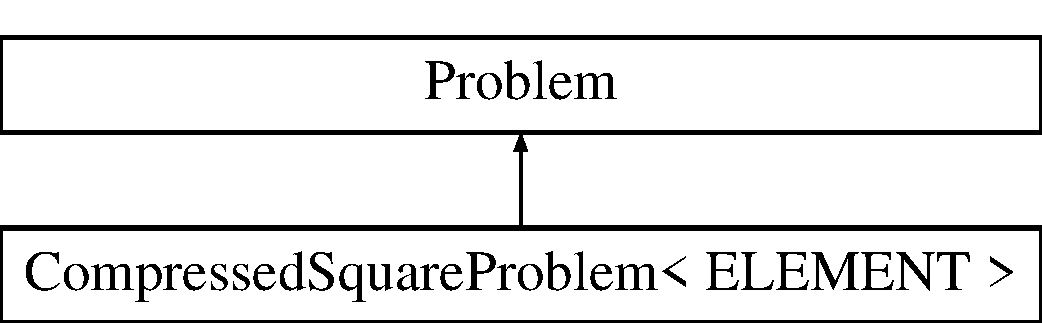
\includegraphics[height=2.000000cm]{classCompressedSquareProblem}
\end{center}
\end{figure}
\subsection*{Public Member Functions}
\begin{DoxyCompactItemize}
\item 
\hyperlink{classCompressedSquareProblem_af013df43f2a9f6ee8ff16cf59ddd9439}{Compressed\+Square\+Problem} (const bool \&incompress)
\begin{DoxyCompactList}\small\item\em Constructor\+: Pass flag that determines if we want to use a true incompressible formulation. \end{DoxyCompactList}\item 
void \hyperlink{classCompressedSquareProblem_afef46d13ff7c8b2845e96a84762077dc}{actions\+\_\+after\+\_\+newton\+\_\+solve} ()
\begin{DoxyCompactList}\small\item\em Update function (empty) \end{DoxyCompactList}\item 
void \hyperlink{classCompressedSquareProblem_aed8338e212b31c56a5df20c222385e15}{actions\+\_\+before\+\_\+newton\+\_\+solve} ()
\begin{DoxyCompactList}\small\item\em Update function (empty) \end{DoxyCompactList}\item 
void \hyperlink{classCompressedSquareProblem_a34d511f377379122d65b2a1402898f5c}{doc\+\_\+solution} (const bool \&incompress)
\begin{DoxyCompactList}\small\item\em Doc the solution \& exact (linear) solution for compressible or incompressible materials. \end{DoxyCompactList}\item 
void \hyperlink{classCompressedSquareProblem_a1543bb8bcba7bf3491e29d141faaf774}{run\+\_\+it} (const int \&i\+\_\+case, const bool \&incompress)
\begin{DoxyCompactList}\small\item\em Run the job -- doc in R\+E\+S\+L\+Ti\+\_\+case. \end{DoxyCompactList}\end{DoxyCompactItemize}
\subsection*{Private Attributes}
\begin{DoxyCompactItemize}
\item 
ofstream \hyperlink{classCompressedSquareProblem_afc8bc8ff7811d18f8d59cd1c35e6cb00}{Trace\+\_\+file}
\begin{DoxyCompactList}\small\item\em Trace file. \end{DoxyCompactList}\item 
Node $\ast$ \hyperlink{classCompressedSquareProblem_a0af6b1044a8392a3ae3d753f4db52664}{Trace\+\_\+node\+\_\+pt}
\begin{DoxyCompactList}\small\item\em Pointers to node whose position we\textquotesingle{}re tracing. \end{DoxyCompactList}\item 
Doc\+Info \hyperlink{classCompressedSquareProblem_a2269691c7bef351c87a4421d275fe7c3}{Doc\+\_\+info}
\begin{DoxyCompactList}\small\item\em Doc\+Info object for output. \end{DoxyCompactList}\end{DoxyCompactItemize}


\subsection{Detailed Description}
\subsubsection*{template$<$class E\+L\+E\+M\+E\+NT$>$\newline
class Compressed\+Square\+Problem$<$ E\+L\+E\+M\+E\+N\+T $>$}

Problem class. 

Definition at line 152 of file compressed\+\_\+square.\+cc.



\subsection{Constructor \& Destructor Documentation}
\mbox{\Hypertarget{classCompressedSquareProblem_af013df43f2a9f6ee8ff16cf59ddd9439}\label{classCompressedSquareProblem_af013df43f2a9f6ee8ff16cf59ddd9439}} 
\index{Compressed\+Square\+Problem@{Compressed\+Square\+Problem}!Compressed\+Square\+Problem@{Compressed\+Square\+Problem}}
\index{Compressed\+Square\+Problem@{Compressed\+Square\+Problem}!Compressed\+Square\+Problem@{Compressed\+Square\+Problem}}
\subsubsection{\texorpdfstring{Compressed\+Square\+Problem()}{CompressedSquareProblem()}}
{\footnotesize\ttfamily template$<$class E\+L\+E\+M\+E\+NT $>$ \\
\hyperlink{classCompressedSquareProblem}{Compressed\+Square\+Problem}$<$ E\+L\+E\+M\+E\+NT $>$\+::\hyperlink{classCompressedSquareProblem}{Compressed\+Square\+Problem} (\begin{DoxyParamCaption}\item[{const bool \&}]{incompress }\end{DoxyParamCaption})}



Constructor\+: Pass flag that determines if we want to use a true incompressible formulation. 

Constructor\+: Pass flag that determines if we want to enforce incompressibility 

Definition at line 193 of file compressed\+\_\+square.\+cc.



References Global\+\_\+\+Physical\+\_\+\+Variables\+::\+Constitutive\+\_\+law\+\_\+pt, and Global\+\_\+\+Physical\+\_\+\+Variables\+::gravity().



\subsection{Member Function Documentation}
\mbox{\Hypertarget{classCompressedSquareProblem_afef46d13ff7c8b2845e96a84762077dc}\label{classCompressedSquareProblem_afef46d13ff7c8b2845e96a84762077dc}} 
\index{Compressed\+Square\+Problem@{Compressed\+Square\+Problem}!actions\+\_\+after\+\_\+newton\+\_\+solve@{actions\+\_\+after\+\_\+newton\+\_\+solve}}
\index{actions\+\_\+after\+\_\+newton\+\_\+solve@{actions\+\_\+after\+\_\+newton\+\_\+solve}!Compressed\+Square\+Problem@{Compressed\+Square\+Problem}}
\subsubsection{\texorpdfstring{actions\+\_\+after\+\_\+newton\+\_\+solve()}{actions\_after\_newton\_solve()}}
{\footnotesize\ttfamily template$<$class E\+L\+E\+M\+E\+NT$>$ \\
void \hyperlink{classCompressedSquareProblem}{Compressed\+Square\+Problem}$<$ E\+L\+E\+M\+E\+NT $>$\+::actions\+\_\+after\+\_\+newton\+\_\+solve (\begin{DoxyParamCaption}{ }\end{DoxyParamCaption})\hspace{0.3cm}{\ttfamily [inline]}}



Update function (empty) 



Definition at line 162 of file compressed\+\_\+square.\+cc.

\mbox{\Hypertarget{classCompressedSquareProblem_aed8338e212b31c56a5df20c222385e15}\label{classCompressedSquareProblem_aed8338e212b31c56a5df20c222385e15}} 
\index{Compressed\+Square\+Problem@{Compressed\+Square\+Problem}!actions\+\_\+before\+\_\+newton\+\_\+solve@{actions\+\_\+before\+\_\+newton\+\_\+solve}}
\index{actions\+\_\+before\+\_\+newton\+\_\+solve@{actions\+\_\+before\+\_\+newton\+\_\+solve}!Compressed\+Square\+Problem@{Compressed\+Square\+Problem}}
\subsubsection{\texorpdfstring{actions\+\_\+before\+\_\+newton\+\_\+solve()}{actions\_before\_newton\_solve()}}
{\footnotesize\ttfamily template$<$class E\+L\+E\+M\+E\+NT$>$ \\
void \hyperlink{classCompressedSquareProblem}{Compressed\+Square\+Problem}$<$ E\+L\+E\+M\+E\+NT $>$\+::actions\+\_\+before\+\_\+newton\+\_\+solve (\begin{DoxyParamCaption}{ }\end{DoxyParamCaption})\hspace{0.3cm}{\ttfamily [inline]}}



Update function (empty) 



Definition at line 165 of file compressed\+\_\+square.\+cc.

\mbox{\Hypertarget{classCompressedSquareProblem_a34d511f377379122d65b2a1402898f5c}\label{classCompressedSquareProblem_a34d511f377379122d65b2a1402898f5c}} 
\index{Compressed\+Square\+Problem@{Compressed\+Square\+Problem}!doc\+\_\+solution@{doc\+\_\+solution}}
\index{doc\+\_\+solution@{doc\+\_\+solution}!Compressed\+Square\+Problem@{Compressed\+Square\+Problem}}
\subsubsection{\texorpdfstring{doc\+\_\+solution()}{doc\_solution()}}
{\footnotesize\ttfamily template$<$class E\+L\+E\+M\+E\+NT $>$ \\
void \hyperlink{classCompressedSquareProblem}{Compressed\+Square\+Problem}$<$ E\+L\+E\+M\+E\+NT $>$\+::doc\+\_\+solution (\begin{DoxyParamCaption}\item[{const bool \&}]{incompress }\end{DoxyParamCaption})}



Doc the solution \& exact (linear) solution for compressible or incompressible materials. 

Doc the solution. 

Definition at line 288 of file compressed\+\_\+square.\+cc.



References Global\+\_\+\+Physical\+\_\+\+Variables\+::\+Gravity, and Global\+\_\+\+Physical\+\_\+\+Variables\+::\+Nu.

\mbox{\Hypertarget{classCompressedSquareProblem_a1543bb8bcba7bf3491e29d141faaf774}\label{classCompressedSquareProblem_a1543bb8bcba7bf3491e29d141faaf774}} 
\index{Compressed\+Square\+Problem@{Compressed\+Square\+Problem}!run\+\_\+it@{run\+\_\+it}}
\index{run\+\_\+it@{run\+\_\+it}!Compressed\+Square\+Problem@{Compressed\+Square\+Problem}}
\subsubsection{\texorpdfstring{run\+\_\+it()}{run\_it()}}
{\footnotesize\ttfamily template$<$class E\+L\+E\+M\+E\+NT $>$ \\
void \hyperlink{classCompressedSquareProblem}{Compressed\+Square\+Problem}$<$ E\+L\+E\+M\+E\+NT $>$\+::run\+\_\+it (\begin{DoxyParamCaption}\item[{const int \&}]{i\+\_\+case,  }\item[{const bool \&}]{incompress }\end{DoxyParamCaption})}



Run the job -- doc in R\+E\+S\+L\+Ti\+\_\+case. 

Run it. 

Definition at line 383 of file compressed\+\_\+square.\+cc.



References Global\+\_\+\+Physical\+\_\+\+Variables\+::\+Gravity.



Referenced by main().



\subsection{Member Data Documentation}
\mbox{\Hypertarget{classCompressedSquareProblem_a2269691c7bef351c87a4421d275fe7c3}\label{classCompressedSquareProblem_a2269691c7bef351c87a4421d275fe7c3}} 
\index{Compressed\+Square\+Problem@{Compressed\+Square\+Problem}!Doc\+\_\+info@{Doc\+\_\+info}}
\index{Doc\+\_\+info@{Doc\+\_\+info}!Compressed\+Square\+Problem@{Compressed\+Square\+Problem}}
\subsubsection{\texorpdfstring{Doc\+\_\+info}{Doc\_info}}
{\footnotesize\ttfamily template$<$class E\+L\+E\+M\+E\+NT$>$ \\
Doc\+Info \hyperlink{classCompressedSquareProblem}{Compressed\+Square\+Problem}$<$ E\+L\+E\+M\+E\+NT $>$\+::Doc\+\_\+info\hspace{0.3cm}{\ttfamily [private]}}



Doc\+Info object for output. 



Definition at line 183 of file compressed\+\_\+square.\+cc.

\mbox{\Hypertarget{classCompressedSquareProblem_afc8bc8ff7811d18f8d59cd1c35e6cb00}\label{classCompressedSquareProblem_afc8bc8ff7811d18f8d59cd1c35e6cb00}} 
\index{Compressed\+Square\+Problem@{Compressed\+Square\+Problem}!Trace\+\_\+file@{Trace\+\_\+file}}
\index{Trace\+\_\+file@{Trace\+\_\+file}!Compressed\+Square\+Problem@{Compressed\+Square\+Problem}}
\subsubsection{\texorpdfstring{Trace\+\_\+file}{Trace\_file}}
{\footnotesize\ttfamily template$<$class E\+L\+E\+M\+E\+NT$>$ \\
ofstream \hyperlink{classCompressedSquareProblem}{Compressed\+Square\+Problem}$<$ E\+L\+E\+M\+E\+NT $>$\+::Trace\+\_\+file\hspace{0.3cm}{\ttfamily [private]}}



Trace file. 



Definition at line 177 of file compressed\+\_\+square.\+cc.

\mbox{\Hypertarget{classCompressedSquareProblem_a0af6b1044a8392a3ae3d753f4db52664}\label{classCompressedSquareProblem_a0af6b1044a8392a3ae3d753f4db52664}} 
\index{Compressed\+Square\+Problem@{Compressed\+Square\+Problem}!Trace\+\_\+node\+\_\+pt@{Trace\+\_\+node\+\_\+pt}}
\index{Trace\+\_\+node\+\_\+pt@{Trace\+\_\+node\+\_\+pt}!Compressed\+Square\+Problem@{Compressed\+Square\+Problem}}
\subsubsection{\texorpdfstring{Trace\+\_\+node\+\_\+pt}{Trace\_node\_pt}}
{\footnotesize\ttfamily template$<$class E\+L\+E\+M\+E\+NT$>$ \\
Node$\ast$ \hyperlink{classCompressedSquareProblem}{Compressed\+Square\+Problem}$<$ E\+L\+E\+M\+E\+NT $>$\+::Trace\+\_\+node\+\_\+pt\hspace{0.3cm}{\ttfamily [private]}}



Pointers to node whose position we\textquotesingle{}re tracing. 



Definition at line 180 of file compressed\+\_\+square.\+cc.



The documentation for this class was generated from the following file\+:\begin{DoxyCompactItemize}
\item 
\hyperlink{compressed__square_8cc}{compressed\+\_\+square.\+cc}\end{DoxyCompactItemize}

\hypertarget{classoomph_1_1MySolidElement}{}\section{oomph\+:\+:My\+Solid\+Element$<$ E\+L\+E\+M\+E\+NT $>$ Class Template Reference}
\label{classoomph_1_1MySolidElement}\index{oomph\+::\+My\+Solid\+Element$<$ E\+L\+E\+M\+E\+N\+T $>$@{oomph\+::\+My\+Solid\+Element$<$ E\+L\+E\+M\+E\+N\+T $>$}}
Inheritance diagram for oomph\+:\+:My\+Solid\+Element$<$ E\+L\+E\+M\+E\+NT $>$\+:\begin{figure}[H]
\begin{center}
\leavevmode
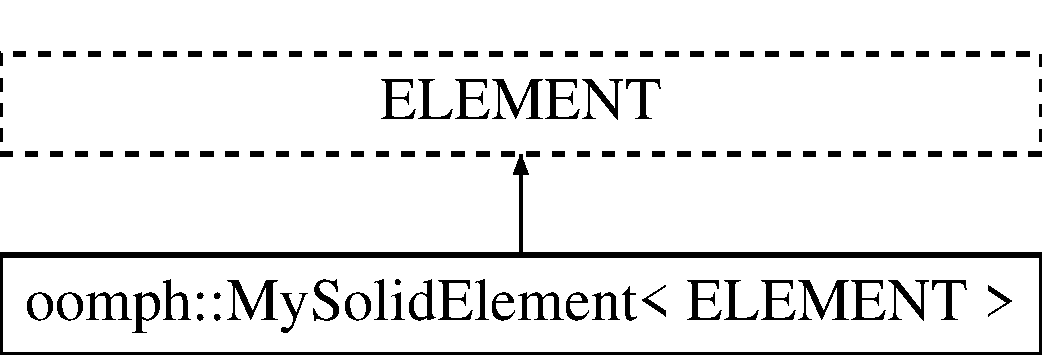
\includegraphics[height=2.000000cm]{classoomph_1_1MySolidElement}
\end{center}
\end{figure}
\subsection*{Public Member Functions}
\begin{DoxyCompactItemize}
\item 
\hyperlink{classoomph_1_1MySolidElement_afe8a392ac0bed5890f64b75adea8f5af}{My\+Solid\+Element} ()
\begin{DoxyCompactList}\small\item\em Constructor\+: Call constructor of underlying element. \end{DoxyCompactList}\item 
void \hyperlink{classoomph_1_1MySolidElement_abf5b903419201b1fd6f1587749337650}{output} (std\+::ostream \&outfile, const unsigned \&n\+\_\+plot)
\begin{DoxyCompactList}\small\item\em Overload output function\+: \end{DoxyCompactList}\item 
\hyperlink{classoomph_1_1MySolidElement_afe8a392ac0bed5890f64b75adea8f5af}{My\+Solid\+Element} ()
\begin{DoxyCompactList}\small\item\em Constructor\+: Call constructor of underlying element. \end{DoxyCompactList}\item 
void \hyperlink{classoomph_1_1MySolidElement_abf5b903419201b1fd6f1587749337650}{output} (std\+::ostream \&outfile, const unsigned \&n\+\_\+plot)
\begin{DoxyCompactList}\small\item\em Overload output function\+: \end{DoxyCompactList}\end{DoxyCompactItemize}


\subsection{Detailed Description}
\subsubsection*{template$<$class E\+L\+E\+M\+E\+NT$>$\newline
class oomph\+::\+My\+Solid\+Element$<$ E\+L\+E\+M\+E\+N\+T $>$}

Wrapper class for solid elements to modify their output functions. 

Definition at line 52 of file airy\+\_\+cantilever.\+cc.



\subsection{Constructor \& Destructor Documentation}
\mbox{\Hypertarget{classoomph_1_1MySolidElement_afe8a392ac0bed5890f64b75adea8f5af}\label{classoomph_1_1MySolidElement_afe8a392ac0bed5890f64b75adea8f5af}} 
\index{oomph\+::\+My\+Solid\+Element@{oomph\+::\+My\+Solid\+Element}!My\+Solid\+Element@{My\+Solid\+Element}}
\index{My\+Solid\+Element@{My\+Solid\+Element}!oomph\+::\+My\+Solid\+Element@{oomph\+::\+My\+Solid\+Element}}
\subsubsection{\texorpdfstring{My\+Solid\+Element()}{MySolidElement()}\hspace{0.1cm}{\footnotesize\ttfamily [1/2]}}
{\footnotesize\ttfamily template$<$class E\+L\+E\+M\+E\+NT $>$ \\
\hyperlink{classoomph_1_1MySolidElement}{oomph\+::\+My\+Solid\+Element}$<$ E\+L\+E\+M\+E\+NT $>$\+::\hyperlink{classoomph_1_1MySolidElement}{My\+Solid\+Element} (\begin{DoxyParamCaption}{ }\end{DoxyParamCaption})\hspace{0.3cm}{\ttfamily [inline]}}



Constructor\+: Call constructor of underlying element. 



Definition at line 58 of file airy\+\_\+cantilever.\+cc.

\mbox{\Hypertarget{classoomph_1_1MySolidElement_afe8a392ac0bed5890f64b75adea8f5af}\label{classoomph_1_1MySolidElement_afe8a392ac0bed5890f64b75adea8f5af}} 
\index{oomph\+::\+My\+Solid\+Element@{oomph\+::\+My\+Solid\+Element}!My\+Solid\+Element@{My\+Solid\+Element}}
\index{My\+Solid\+Element@{My\+Solid\+Element}!oomph\+::\+My\+Solid\+Element@{oomph\+::\+My\+Solid\+Element}}
\subsubsection{\texorpdfstring{My\+Solid\+Element()}{MySolidElement()}\hspace{0.1cm}{\footnotesize\ttfamily [2/2]}}
{\footnotesize\ttfamily template$<$class E\+L\+E\+M\+E\+NT $>$ \\
\hyperlink{classoomph_1_1MySolidElement}{oomph\+::\+My\+Solid\+Element}$<$ E\+L\+E\+M\+E\+NT $>$\+::\hyperlink{classoomph_1_1MySolidElement}{My\+Solid\+Element} (\begin{DoxyParamCaption}{ }\end{DoxyParamCaption})\hspace{0.3cm}{\ttfamily [inline]}}



Constructor\+: Call constructor of underlying element. 



Definition at line 60 of file airy\+\_\+cantilever2.\+cc.



\subsection{Member Function Documentation}
\mbox{\Hypertarget{classoomph_1_1MySolidElement_abf5b903419201b1fd6f1587749337650}\label{classoomph_1_1MySolidElement_abf5b903419201b1fd6f1587749337650}} 
\index{oomph\+::\+My\+Solid\+Element@{oomph\+::\+My\+Solid\+Element}!output@{output}}
\index{output@{output}!oomph\+::\+My\+Solid\+Element@{oomph\+::\+My\+Solid\+Element}}
\subsubsection{\texorpdfstring{output()}{output()}\hspace{0.1cm}{\footnotesize\ttfamily [1/2]}}
{\footnotesize\ttfamily template$<$class E\+L\+E\+M\+E\+NT $>$ \\
void \hyperlink{classoomph_1_1MySolidElement}{oomph\+::\+My\+Solid\+Element}$<$ E\+L\+E\+M\+E\+NT $>$\+::output (\begin{DoxyParamCaption}\item[{std\+::ostream \&}]{outfile,  }\item[{const unsigned \&}]{n\+\_\+plot }\end{DoxyParamCaption})\hspace{0.3cm}{\ttfamily [inline]}}



Overload output function\+: 



Definition at line 61 of file airy\+\_\+cantilever.\+cc.

\mbox{\Hypertarget{classoomph_1_1MySolidElement_abf5b903419201b1fd6f1587749337650}\label{classoomph_1_1MySolidElement_abf5b903419201b1fd6f1587749337650}} 
\index{oomph\+::\+My\+Solid\+Element@{oomph\+::\+My\+Solid\+Element}!output@{output}}
\index{output@{output}!oomph\+::\+My\+Solid\+Element@{oomph\+::\+My\+Solid\+Element}}
\subsubsection{\texorpdfstring{output()}{output()}\hspace{0.1cm}{\footnotesize\ttfamily [2/2]}}
{\footnotesize\ttfamily template$<$class E\+L\+E\+M\+E\+NT $>$ \\
void \hyperlink{classoomph_1_1MySolidElement}{oomph\+::\+My\+Solid\+Element}$<$ E\+L\+E\+M\+E\+NT $>$\+::output (\begin{DoxyParamCaption}\item[{std\+::ostream \&}]{outfile,  }\item[{const unsigned \&}]{n\+\_\+plot }\end{DoxyParamCaption})\hspace{0.3cm}{\ttfamily [inline]}}



Overload output function\+: 



Definition at line 63 of file airy\+\_\+cantilever2.\+cc.



The documentation for this class was generated from the following files\+:\begin{DoxyCompactItemize}
\item 
\hyperlink{airy__cantilever_8cc}{airy\+\_\+cantilever.\+cc}\item 
\hyperlink{airy__cantilever2_8cc}{airy\+\_\+cantilever2.\+cc}\end{DoxyCompactItemize}

\chapter{File Documentation}
\hypertarget{compressed__square_8cc}{}\section{compressed\+\_\+square.\+cc File Reference}
\label{compressed__square_8cc}\index{compressed\+\_\+square.\+cc@{compressed\+\_\+square.\+cc}}
\subsection*{Classes}
\begin{DoxyCompactItemize}
\item 
class \hyperlink{classoomph_1_1MySolidElement}{oomph\+::\+My\+Solid\+Element$<$ E\+L\+E\+M\+E\+N\+T $>$}
\begin{DoxyCompactList}\small\item\em Wrapper class for solid element to modify the output. \end{DoxyCompactList}\item 
class \hyperlink{classCompressedSquareProblem}{Compressed\+Square\+Problem$<$ E\+L\+E\+M\+E\+N\+T $>$}
\begin{DoxyCompactList}\small\item\em Problem class. \end{DoxyCompactList}\end{DoxyCompactItemize}
\subsection*{Namespaces}
\begin{DoxyCompactItemize}
\item 
 \hyperlink{namespaceoomph}{oomph}
\item 
 \hyperlink{namespaceGlobal__Physical__Variables}{Global\+\_\+\+Physical\+\_\+\+Variables}
\begin{DoxyCompactList}\small\item\em Global variables. \end{DoxyCompactList}\end{DoxyCompactItemize}
\subsection*{Functions}
\begin{DoxyCompactItemize}
\item 
void \hyperlink{namespaceGlobal__Physical__Variables_a0777aef63372db7f91ad894c38159681}{Global\+\_\+\+Physical\+\_\+\+Variables\+::gravity} (const double \&time, const Vector$<$ double $>$ \&xi, Vector$<$ double $>$ \&b)
\begin{DoxyCompactList}\small\item\em Non-\/dimensional gravity as body force. \end{DoxyCompactList}\item 
int \hyperlink{compressed__square_8cc_ae66f6b31b5ad750f1fe042a706a4e3d4}{main} ()
\begin{DoxyCompactList}\small\item\em Driver for compressed square. \end{DoxyCompactList}\end{DoxyCompactItemize}
\subsection*{Variables}
\begin{DoxyCompactItemize}
\item 
Constitutive\+Law $\ast$ \hyperlink{namespaceGlobal__Physical__Variables_a2a37fb040c832ee7a086bb13bb02a100}{Global\+\_\+\+Physical\+\_\+\+Variables\+::\+Constitutive\+\_\+law\+\_\+pt} =0
\begin{DoxyCompactList}\small\item\em Pointer to constitutive law. \end{DoxyCompactList}\item 
double \hyperlink{namespaceGlobal__Physical__Variables_a3962c36313826b19f216f6bbbdd6a477}{Global\+\_\+\+Physical\+\_\+\+Variables\+::\+Nu} =0.\+45
\begin{DoxyCompactList}\small\item\em Poisson\textquotesingle{}s ratio for Hooke\textquotesingle{}s law. \end{DoxyCompactList}\item 
Strain\+Energy\+Function $\ast$ \hyperlink{namespaceGlobal__Physical__Variables_a73135f793690b4386bf83bbefc7bf310}{Global\+\_\+\+Physical\+\_\+\+Variables\+::\+Strain\+\_\+energy\+\_\+function\+\_\+pt} =0
\begin{DoxyCompactList}\small\item\em Pointer to strain energy function. \end{DoxyCompactList}\item 
double \hyperlink{namespaceGlobal__Physical__Variables_a849754fa7155c1a31481674ce4845658}{Global\+\_\+\+Physical\+\_\+\+Variables\+::\+C1} =1.\+3
\begin{DoxyCompactList}\small\item\em First \char`\"{}\+Mooney Rivlin\char`\"{} coefficient for generalised Mooney Rivlin law. \end{DoxyCompactList}\item 
double \hyperlink{namespaceGlobal__Physical__Variables_af9defd1b5745cce50d2c386b3ac0e0ae}{Global\+\_\+\+Physical\+\_\+\+Variables\+::\+C2} =1.\+3
\begin{DoxyCompactList}\small\item\em Second \char`\"{}\+Mooney Rivlin\char`\"{} coefficient for generalised Mooney Rivlin law. \end{DoxyCompactList}\item 
double \hyperlink{namespaceGlobal__Physical__Variables_a8b80d3e8d63b8d0a0ed435a2dd7fe2ad}{Global\+\_\+\+Physical\+\_\+\+Variables\+::\+Gravity} =0.\+0
\begin{DoxyCompactList}\small\item\em Non-\/dim gravity. \end{DoxyCompactList}\end{DoxyCompactItemize}


\subsection{Function Documentation}
\mbox{\Hypertarget{compressed__square_8cc_ae66f6b31b5ad750f1fe042a706a4e3d4}\label{compressed__square_8cc_ae66f6b31b5ad750f1fe042a706a4e3d4}} 
\index{compressed\+\_\+square.\+cc@{compressed\+\_\+square.\+cc}!main@{main}}
\index{main@{main}!compressed\+\_\+square.\+cc@{compressed\+\_\+square.\+cc}}
\subsubsection{\texorpdfstring{main()}{main()}}
{\footnotesize\ttfamily int main (\begin{DoxyParamCaption}{ }\end{DoxyParamCaption})}



Driver for compressed square. 



Definition at line 425 of file compressed\+\_\+square.\+cc.



References Global\+\_\+\+Physical\+\_\+\+Variables\+::\+C1, Global\+\_\+\+Physical\+\_\+\+Variables\+::\+C2, Global\+\_\+\+Physical\+\_\+\+Variables\+::\+Constitutive\+\_\+law\+\_\+pt, Global\+\_\+\+Physical\+\_\+\+Variables\+::\+Nu, Compressed\+Square\+Problem$<$ E\+L\+E\+M\+E\+N\+T $>$\+::run\+\_\+it(), and Global\+\_\+\+Physical\+\_\+\+Variables\+::\+Strain\+\_\+energy\+\_\+function\+\_\+pt.


\hypertarget{compressed__square_8txt__doxygenified_8h}{}\section{compressed\+\_\+square.\+txt\+\_\+doxygenified.\+h File Reference}
\label{compressed__square_8txt__doxygenified_8h}\index{compressed\+\_\+square.\+txt\+\_\+doxygenified.\+h@{compressed\+\_\+square.\+txt\+\_\+doxygenified.\+h}}

%--- End generated contents ---

% Index
\backmatter
\newpage
\phantomsection
\clearemptydoublepage
\addcontentsline{toc}{chapter}{Index}
\printindex

\end{document}
